\tikzsetnextfilename{fbd2}
\begin{center}
   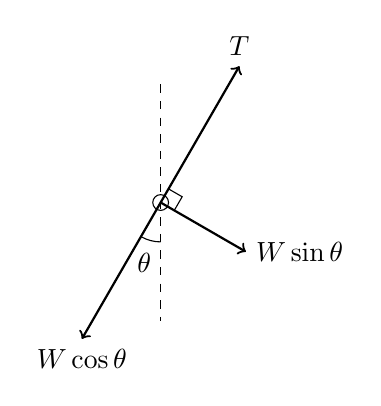
\begin{tikzpicture}

      % Definitions
      \def\angle{-120}  % Angle of string
      \def\br{0.1}      % Radius of bob
      \def\dh{1.5}      % Half-height of dashed line
      \def\lT{2}        % Length of the T and W cos theta vectors
      \def\ln{0.2}      % Lenght of 90 degree box
      \def\ar{0.5}     % Radius of angle arc
      \def\tangle{ {(\angle - 90) / 2} }      % Calculate the angle between -90 and \angle for placing the \theta symbol. Note the use of extra {} to encapsulate the calculation

      \coordinate (O) at (0,0);

      % Draw commands
      \draw (O) circle [radius=\br];
      \draw [dashed] (0,\dh) -- (0,-\dh);

      \draw [->, thick] (O) -- ++ (\angle:\lT) node [below] {$W \cos \theta$};
      \draw [->, thick] (O) -- ++ (\angle+180:\lT) node [above] {$T$};
      \draw [->, thick] (O) -- ++ (\angle+90:1.25) node [anchor=west] {$W \sin \theta$};

      \draw (\angle+180:\ln) -- ++ (\angle+90:\ln) -- ++ (\angle:\ln);      % Small box representing a 90 degree angle between T and W sin\theta
      \draw (-90:\ar) arc (-90:\angle:\ar);
      \draw (\tangle:\ar+0.3) node {$\theta$};

   \end{tikzpicture}
\end{center}
